% !TEX spellcheck = en_US
% !TeX root = Lecture.tex
%---------------------------------------------------------------------------------
\section[Introduction]{}\label{sec:INT}
%---------------------------------------------------------------------------------
\begin{frame}{How large is the largest wind turbine blade?}
	\centering 
	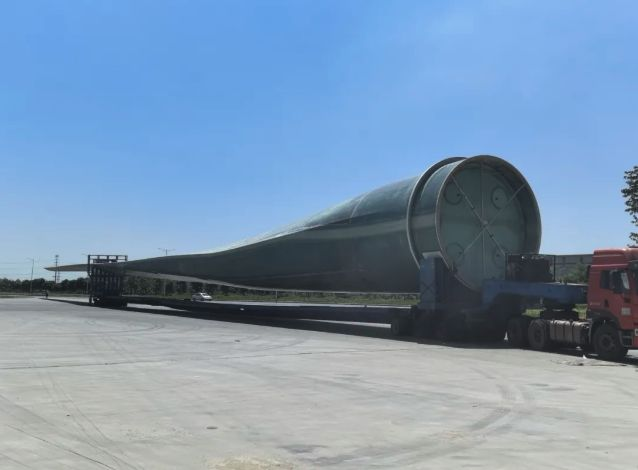
\includegraphics[height=4.0cm]{INT/Sinoma}
	\hspace{0.3cm}
	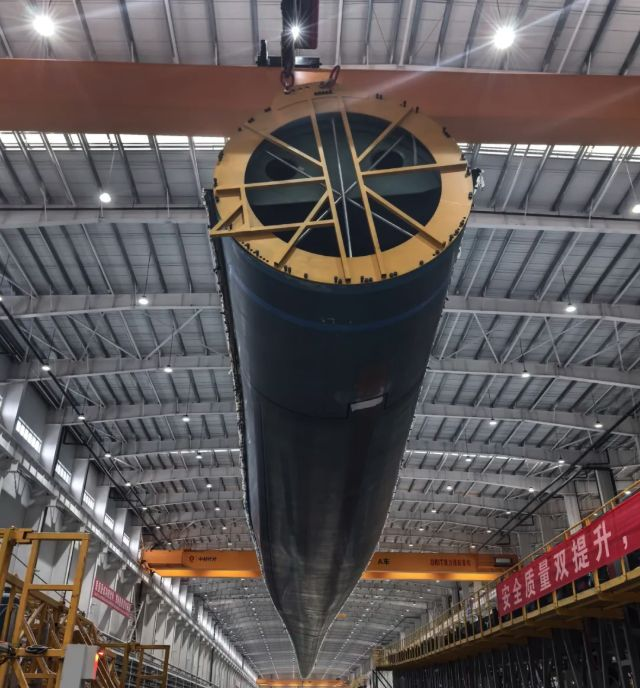
\includegraphics[height=4.0cm]{INT/Sinoma2}\\
	{\tiny\textcolor{gray}{[http://yp.sinomatech.com/en/news/10401.html/]}}
	\begin{block}<2->{Sinoma's 147-meter blade successfully passes the static test verification}
	\small News from 09-29-2024: 	The GW147 blade is an ultra-long blade specially designed for offshore wind power generation. The blade is 147 m long with a rated power of 20 MW. During the trial production process, the R\&D personnel of Goldwind and Sinoma Blade worked together and relied on top-notch mechanized and automated equipment for process planning.
	\end{block}	
\end{frame}
%---------------------------------------------------------------------------------
\begin{frame}{How can we design a wind turbine blade?} 
	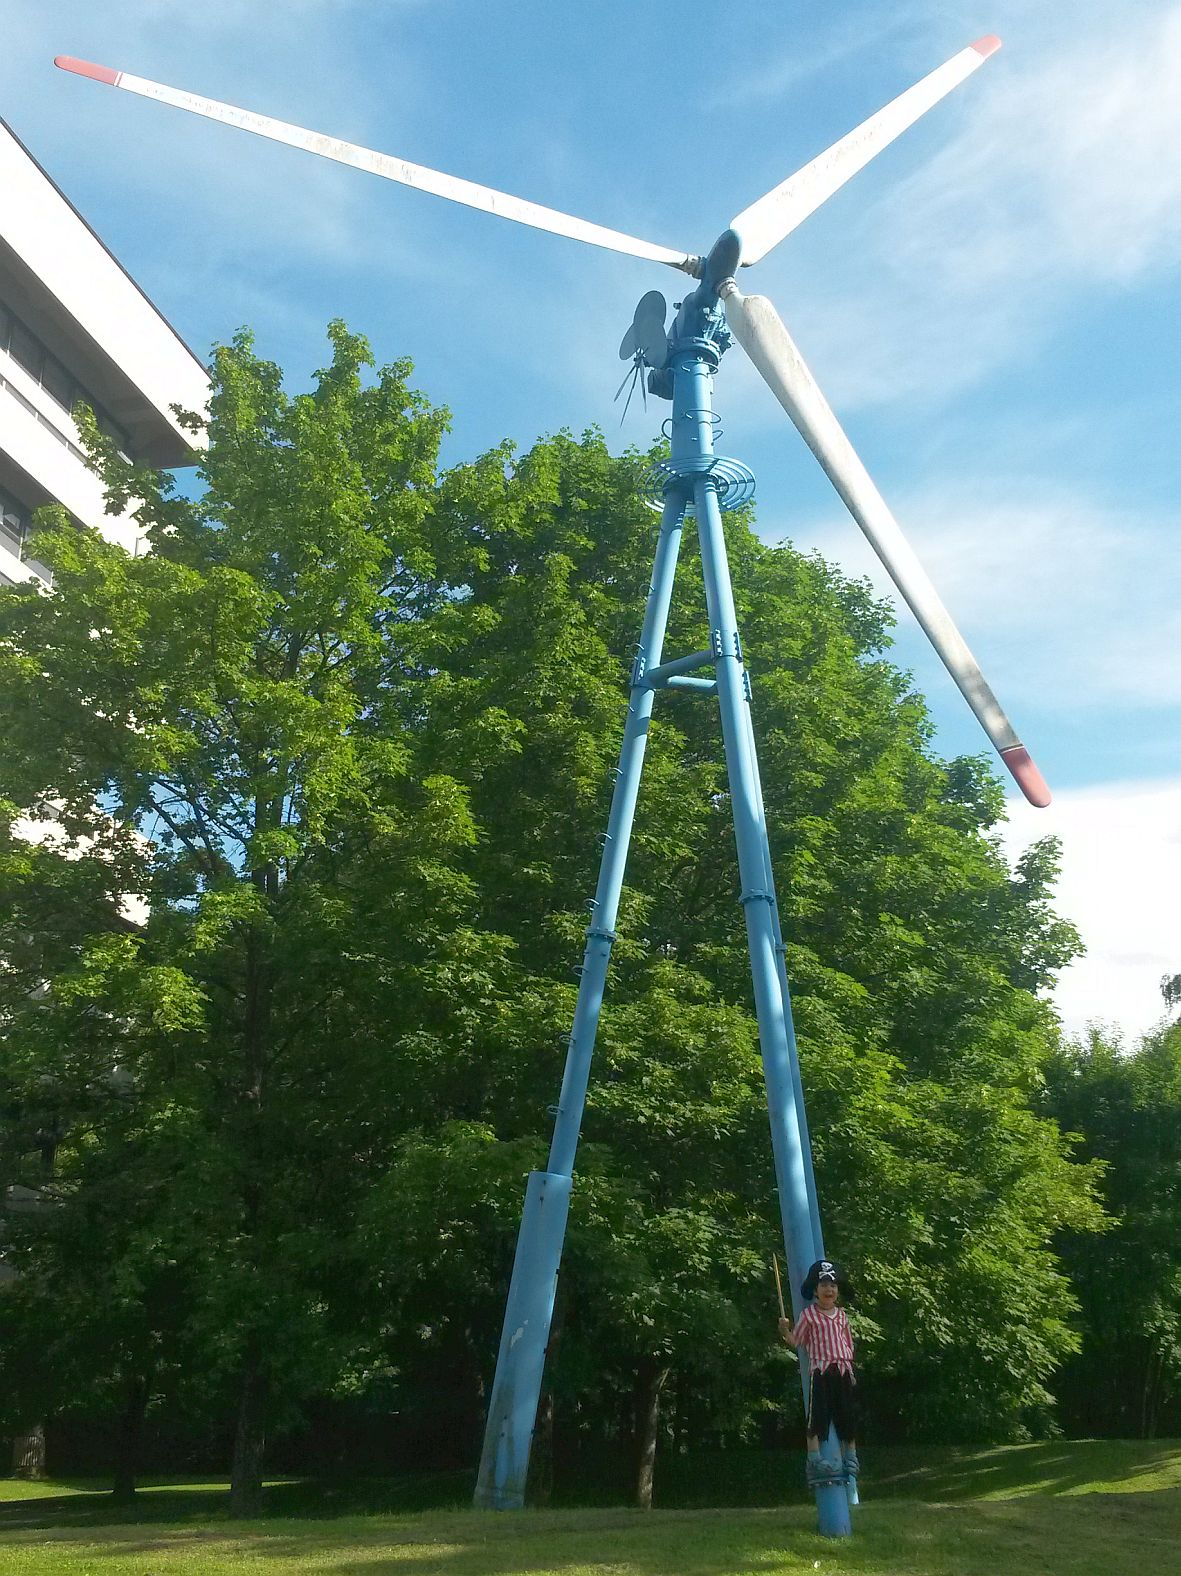
\includegraphics[width=4.0cm]{INT/IFBHuetter_600DPI}%
	\hskip 0.10cm
	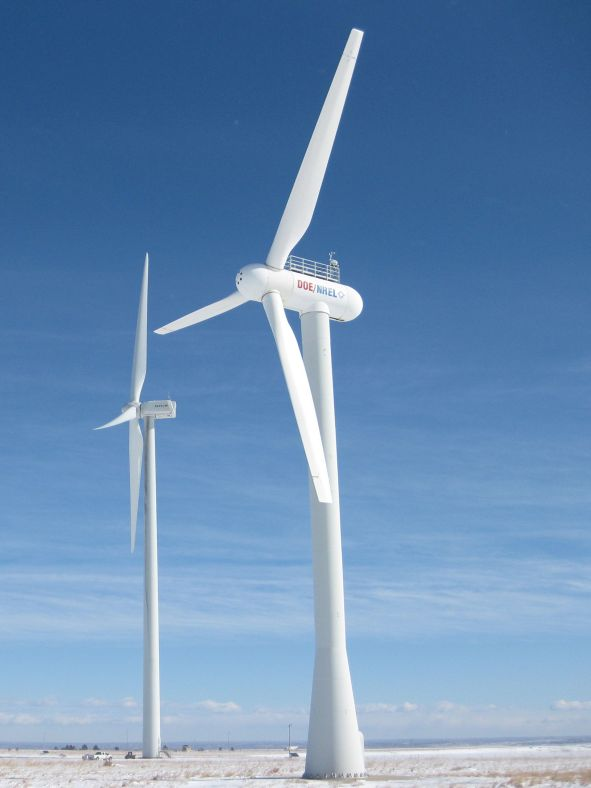
\includegraphics[width=4.0cm]{INT/NRELCART3}%
	\hskip 0.10cm
	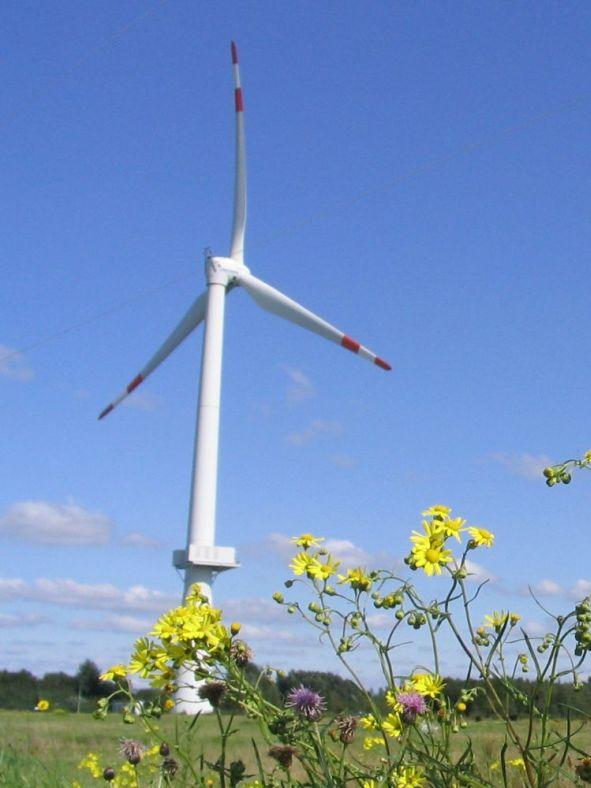
\includegraphics[width=4.0cm]{INT/M5000}%				
	\visible<2->{
	\begin{alertblock}{Main questions today}
		\begin{itemize}
			\item How much wind energy can be extracted theoretically by a wind turbine?
			\item How does this help us to design an optimal wind turbine blade?
		\end{itemize}
	\end{alertblock}
	}
\end{frame}
%---------------------------------------------------------------------------------
\begin{frame}{Learning objectives}  	
\begin{block}{After this lectures you should be able to...}
	\begin{itemize}
		\item explain, how much kinetic energy is in the wind and which maximum fraction of this energy can be converted to mechanical energy
		\item derive the maximum power coefficient according to Betz
		\item select values for rotor design from an airfoil
		\item design a rotor according to Betz
	\end{itemize}
\end{block}
\end{frame}
%---------------------------------------------------------------------------------
\begin{frame}{Content}
\tableofcontents
\PutAt<1->[5cm]{(10cm,2cm)}{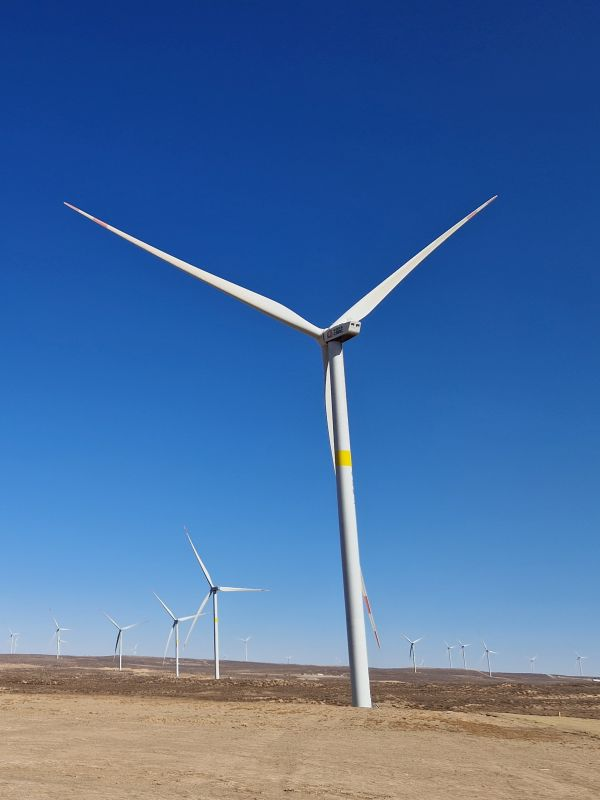
\includegraphics[width=4.0cm]{\StylePath/content/Gobi}} % graphic related to topic	
\end{frame}
%---------------------------------------------------------------------------------


